\documentclass[11pt]{article}

\usepackage[margin=1in]{geometry}
\usepackage{parskip}
\setlength{\emergencystretch}{4em}   % absorb unbreakable \texttt{} long tokens
\hyphenation{from-Extension-Path-Optimized Polyhedron-View Deltahedron-View}
\usepackage{booktabs}
\usepackage{longtable}
\usepackage{xcolor}
\usepackage{listings}
\usepackage{enumitem}
\usepackage[hidelinks]{hyperref}
\usepackage{tikz}
\usetikzlibrary{arrows.meta,positioning}

\definecolor{kw}{rgb}{0.15,0.15,0.55}
\definecolor{cm}{rgb}{0.35,0.45,0.35}
\definecolor{st}{rgb}{0.55,0.20,0.20}
\definecolor{bg}{rgb}{0.975,0.975,0.97}

\lstdefinestyle{py}{
  language=Python, basicstyle=\ttfamily\small, backgroundcolor=\color{bg},
  keywordstyle=\color{kw}, commentstyle=\color{cm}\itshape, stringstyle=\color{st},
  showstringspaces=false, columns=fullflexible, breaklines=true,
  frame=single, framerule=0pt, framesep=6pt, xleftmargin=4pt, aboveskip=8pt, belowskip=8pt,
  morekeywords={fl}}
\lstdefinestyle{sh}{basicstyle=\ttfamily\small, backgroundcolor=\color{bg},
  commentstyle=\color{cm}\itshape, showstringspaces=false, columns=fullflexible,
  breaklines=true, frame=single, framerule=0pt, framesep=6pt, xleftmargin=4pt}
\lstset{style=py}
\newcommand{\code}[1]{\lstinline[style=py]!#1!}

\title{\textbf{The \texttt{fullerenes} Python interface}\\[2pt]
\large A zero-copy \texttt{pybind11} binding with a generated, drift-gated surface}
\author{Fullerenes project --- \texttt{src/pybind}}
\date{June 2026}

\begin{document}
\maketitle

\begin{abstract}
\noindent
\texttt{fullerenes} is a Python extension over the C\texttt{++}/SYCL fullerene library
(\texttt{libfullerenes.so}). It exposes topology, geometry, optimisation, isomer
enumeration, canonical naming and symmetry for fullerene cages, and it is built on the
library's \emph{view\,+\,owned} memory architecture so that numpy arrays and the C\texttt{++}
algorithms share a single allocation --- there is no marshalling on the hot path. The
mechanical method surface is \emph{generated from the clang AST} of the library headers
rather than hand-typed, and two fail-closed drift gates keep both the compiled bindings
and the type stubs in lock-step with the C\texttt{++} API. This report describes the
public interface, how to use it, and how it is generated and guarded.
\end{abstract}

\tableofcontents

\section{Overview}

The binding is a thin, type-safe Python layer (\autoref{tab:classes}) over the existing
C\texttt{++} library. Its design goal is \emph{one representation, two ownership modes,
zero copies on the hot path}: a fullerene's adjacency and coordinates live in exactly one
buffer, and Python sees that buffer directly as numpy arrays. Nothing is re-implemented in
the binding --- every operation materialises a trivially-copyable C\texttt{++} \emph{view}
over the live storage and calls the real library method.

\begin{table}[h]
\centering\small
\begin{tabular}{@{}lll@{}}
\toprule
Class / function & Role & Backing \\
\midrule
\texttt{FullereneGraph}  & cubic ($3$-valent) cage graph         & \texttt{int32 (N,3)} adjacency \\
\texttt{FullereneDual}   & dual triangulation (deg $5$/$6$)      & \texttt{int32 (N,6)} adjacency \\
\texttt{Polyhedron}      & graph $+$ \texttt{float64 (N,3)} 3D coords & adjacency $+$ points \\
\texttt{Deltahedron}     & equilateral-triangle dual embedding   & adjacency $+$ points \\
\texttt{Symmetry}        & point group, orbits, $3$D representation & (from a dual) \\
\texttt{IsomerDB}, \texttt{IsomerEntry} & on-disk isomer database access & files \\
\texttt{BuckyGenerator}  & lazy iterator over all size-$N$ isomers & buckygen subprocess \\
\addlinespace
\texttt{number\_isomers}, \texttt{symmetries} & file-free counts / point-group lists & hard-coded tables \\
\texttt{buckygen}        & enumerate isomers as \texttt{FullereneDual} & --- \\
\texttt{set/get\_database\_path} & configure the database location & --- \\
\bottomrule
\end{tabular}
\caption{The public surface (the full signatures are in \texttt{fullerenes/\_fullerenes.pyi}).}
\label{tab:classes}
\end{table}

\paragraph{Scope.} The interface covers the CPU single-graph API. The GPU/SYCL
\emph{batch} pipeline is intentionally out of scope for this version.

\section{Architecture: view, owned, and the two modes}
\label{sec:arch}

\subsection{View and owned in the library}
The library factors every graph/geometry type into a trivially-copyable \emph{view}
(just \texttt{std::span}s and a few scalars) and an \emph{owned} layer that adds
\texttt{std::vector} storage:
\begin{center}\small\ttfamily
GraphView $\to$ PlanarGraphView $\to$ \{CubicGraphView $\to$ FullereneGraphView\}\\
\phantom{GraphView $\to$ PlanarGraphView $\to$}\,\,$\to$ \{TriangulationView $\to$ FullereneDualView\}
\end{center}
Geometry views (\texttt{PolyhedronView<double>}, \texttt{DeltahedronView<double>}) add a
\texttt{span<coord3d> points}. An \emph{owned} object \textsc{is-a} view, so every
\texttt{const SomeView\&} library entry point accepts an owned object directly, and library
factories (\texttt{dual\_graph}, \texttt{GCtransform}, \texttt{fromExtensionPathOptimized},
\ldots) return owned objects by value.

\subsection{The wrapper: one type, two modes}
Each Python class is a thin C\texttt{++} wrapper --- \code{PyGraph<Owned,View>} (adjacency)
or \code{PyGeom<Owned,View>} (adjacency $+$ \texttt{points}; \code{PyGeom} derives
\code{PyGraph}) --- in one of two modes:

\begin{description}[leftmargin=1.4em]
\item[Owned mode] (the library produced it): the wrapper holds an \texttt{Owned<View>} by
  value. \code{.neighbours}, \code{.deg}, \code{.points} are returned as zero-copy
  \code{py::array_t(shape, strides, ptr, base=self)} views into the owned vectors; the
  \texttt{base=self} keep-alive ties the numpy array's lifetime to the wrapper, so there is
  no copy and no dangling.
\item[View mode] (bring-your-own-buffer): the wrapper holds the caller's numpy arrays as
  keep-alive references; \code{view()} rebuilds a bare \texttt{*View} over their data
  pointers on each call. In-place algorithms (\code{optimize}, \code{reflect},
  \code{move}, \code{scale}, \code{align\_with\_axes}) write \emph{straight back} into the
  caller's array.
\end{description}

A one-line \code{enum Mode} discriminates the two; there is no \texttt{std::variant}.

\subsection{The reallocation invariant}
The safety of the zero-copy views rests on one rule: \textbf{a wrapper's backing storage
never reallocates in place.} Only value-writing in-place mutators are bound as
\texttt{self}-methods. Any operation that changes \texttt{N} or \texttt{dmax}
(\code{resize}, \code{apply\_permutation}, \code{remove\_*}, the GC/Halma/leapfrog
transforms, \code{dual}, \code{convex\_hull}, \ldots) is exposed as a function that returns
a \emph{new} wrapper, so outstanding numpy views can never dangle.

\subsection{Memory layout is contractual}
The zero-copy views are valid only because the C\texttt{++} PODs match the numpy dtypes
exactly (\autoref{tab:layout}); these are guarded by \code{static_assert}s in
\texttt{np\_interop.hh}.

\begin{table}[h]
\centering\small
\begin{tabular}{@{}llll@{}}
\toprule
C\texttt{++} type & size & numpy & meaning \\
\midrule
\texttt{node\_t}            & 4 B  & \texttt{int32}            & vertex id \\
\texttt{neighbours} (flat)  & --   & \texttt{int32 (N,dmax)}   & row-major; cols $\ge$ \texttt{deg[u]} are $-1$ \\
\texttt{deg}                & 1 B  & \texttt{uint8 (N,)}       & per-vertex degree \\
\texttt{coord3d}            & 24 B & \texttt{float64 (N,3)}    & 3D coordinate \\
\texttt{tri\_t}             & 12 B & \texttt{int32 (F,3)}      & triangle \\
\texttt{matrix3d}           & 72 B & \texttt{float64 (3,3)}    & $3\times3$ matrix \\
\bottomrule
\end{tabular}
\caption{POD$\to$dtype contract. \code{.neighbours} is the raw padded view;
\code{.adjacency()} is the clean ragged copy (padding stripped).}
\label{tab:layout}
\end{table}

\section{Using the interface}
\label{sec:usage}

Import is just \code{import fullerenes as fl}. The package re-exports the extension and
sets a default database path if present.

\subsection{Enumeration and canonical names}
\begin{lstlisting}
import fullerenes as fl

# Lazily enumerate every C60 isomer as a dual triangulation:
for dual in fl.buckygen(60):
    name = dual.name()           # canonical: "C60-[GS:1,7,9,...]-fullerene"
    if dual.is_a_fullerene():
        cubic = dual.dual()      # back to the 3-valent cage graph

# Counts and point groups need no database:
fl.number_isomers(60)            # 1812
fl.number_isomers(60, IPR=True)  # 1
fl.symmetries(60)                # ['C1', 'C2', ..., 'Ih']
\end{lstlisting}
The canonical name is invariant under vertex relabelling and stable across enumerator
versions, so it is the right primary key for cross-referencing isomers. A name round-trips
through \code{FullereneDual.from_rspi(N, rspi, jumps)}.

\subsection{Zero-copy accessors (owned mode)}
\begin{lstlisting}
fg = fl.FullereneGraph.C20()
nb = fg.neighbours               # int32 (12, 3) view, NOT a copy
assert nb.base is fg             # keep-alive: fg stays alive while nb does
assert nb.flags.owns_data is False
adj = fg.adjacency()             # ragged list[list[int]] copy (padding removed)
\end{lstlisting}

\subsection{Bring-your-own-buffer and in-place write-back}
\begin{lstlisting}
import numpy as np
# Wrap caller-owned numpy arrays with NO copy (validated dtype/shape/contiguity):
P = fl.Polyhedron.from_arrays(neighbours, points)   # int32 (N,3) + float64 (N,3)
ptr = points.__array_interface__['data'][0]
P.optimize()                     # force-field relaxation writes into `points`
assert points.__array_interface__['data'][0] == ptr   # same buffer, new contents
V = P.volume()                   # reflects whatever is in `points`
\end{lstlisting}

\subsection{Equilateral embeddings (Deltahedron)}
\begin{lstlisting}
D = fl.Deltahedron.from_dual(fl.FullereneGraph.C20().dual())
assert D.count_concave() == 0 and D.max_angle_relerr() < 1e-6   # C20 = icosahedron
r = D.optimize()                 # r in {CONVERGED, STAGNATED, ...}
D.final_opt_result, D.iterations_used, D.final_gmax_L     # snapshot of the last run
\end{lstlisting}
\code{from\_dual} runs the reduction/expansion pipeline
(\texttt{ReducibleDual} $\to$ \texttt{reduceToExtensionPath} $\to$ \texttt{fromExtensionPathOptimized})
and returns an already-optimised embedding. The \code{final\_*} / \code{iterations\_used}
attributes are a snapshot of the last \code{optimize}/\code{from\_dual}; reading one before
any run \emph{raises} rather than returning a fabricated verdict.

\subsection{Symmetry, database, surface geodesics}
\begin{lstlisting}
sym = fl.Symmetry(dual)
sym.point_group()                # 'Ih'
sym.order()                      # 120
sym.equivalence_classes()        # vertex orbits, list[list[int]]
sym.representation_3d()          # (order, 3, 3) float64 O(3) matrices

fl.set_database_path("~/fullerene-data/database")
db = fl.IsomerDB.read(60)        # all 1812 C60 isomers
db[0].group, db[0].rspi, db[0].hlgap
g  = db.make_isomer(0)           # -> FullereneGraph

# Intrinsic-metric surface distances over the dual:
dual.surface_distances()         # (n,n) float64 geodesic distances
\end{lstlisting}
Symmetry (the assignment of $O(3)$ matrices to combinatorial automorphisms) is derived
\emph{purely from graph combinatorics}, never from $3$D coordinates.

\section{How the binding surface is generated}
\label{sec:gen}

The C\texttt{++} API changes often, so the \emph{method surface} is generated from the
clang AST instead of hand-typed. The generator (\texttt{tools/gen\_bindings.py}) follows the
in-project precedent \texttt{buckygen-revival/tools/extract\_bucky\_c.py} and is
\emph{fail-closed}: anything it cannot classify is reported, never silently dropped.

\begin{figure}[h]
\centering
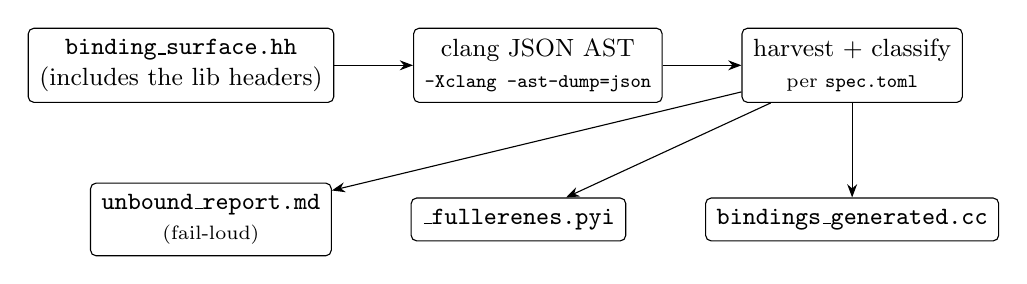
\begin{tikzpicture}[node distance=6mm and 10mm, every node/.style={font=\small},
  box/.style={draw, rounded corners=2pt, align=center, inner sep=4pt}]
\node[box] (surf) {\texttt{binding\_surface.hh}\\(includes the lib headers)};
\node[box, right=of surf] (ast) {clang JSON AST\\\scriptsize\texttt{-Xclang -ast-dump=json}};
\node[box, right=of ast] (cls) {harvest $+$ classify\\\scriptsize per \texttt{spec.toml}};
\node[box, below=12mm of cls] (cc) {\texttt{bindings\_generated.cc}};
\node[box, left=of cc] (pyi) {\texttt{\_fullerenes.pyi}};
\node[box, left=of pyi] (rep) {\texttt{unbound\_report.md}\\\scriptsize(fail-loud)};
\draw[-{Stealth}] (surf)--(ast); \draw[-{Stealth}] (ast)--(cls);
\draw[-{Stealth}] (cls)--(cc); \draw[-{Stealth}] (cls)--(pyi); \draw[-{Stealth}] (cls)--(rep);
\end{tikzpicture}
\caption{The generation pipeline. One pure function \code{generate(AST, spec)} produces
all three artifacts; the committed files are its fixpoint.}
\label{fig:gen}
\end{figure}

\subsection{The pipeline}
\begin{enumerate}[leftmargin=1.6em]
\item \textbf{Dump.} \code{clang++ -std=gnu++23 -Xclang -ast-dump=json} on
  \texttt{tools/binding\_surface.hh} (which \texttt{\#include}s the library headers to bind).
  The AST --- never a text parser --- is the single source of truth.
\item \textbf{Harvest.} For each \texttt{[[klass]]} in \texttt{spec.toml}, walk the C\texttt{++}
  view chain (leaf first; a leaf method \emph{hides} a base method of the same name, matching
  C\texttt{++} name-hiding) and collect the public methods.
\item \textbf{Classify.} Each method's return/parameter types are matched against a fixed
  rule table: scalars ($\to$ \texttt{int}/\texttt{float}/\texttt{bool}), strings,
  \texttt{coord3<T>}/\texttt{matrix3d}/\texttt{tri\_t}/\texttt{face\_t} ($\to$ numpy copies via
  \texttt{np\_interop}), and \emph{owned} return types ($\to$ a cross-class \texttt{Py*}
  wrapper). A method that does not fit any rule, or takes an unsupported parameter, goes to
  the report.
\item \textbf{Dead-declaration gate.} A method declared in a header but \emph{not defined}
  in \texttt{libfullerenes.so} would make the module fail to import. The generator reads the
  built \texttt{.so} with \code{nm -DC --defined-only} and refuses to bind a nullary method
  whose exact \texttt{Class::method} symbol is absent.
\item \textbf{Emit.} \texttt{bindings\_generated.cc} (one
  \texttt{register\_generated\_<Class>(cls)} per class), \texttt{\_fullerenes.pyi} (type
  stubs), and \texttt{unbound\_report.md} (every unclassifiable method, with its reason).
\end{enumerate}

\subsection{\texttt{spec.toml}: what to bind, and the hand-written stubs}
\texttt{spec.toml} is the generator's data file. A \texttt{[[klass]]} names the owned/view
types, the \texttt{harvest} chain, a \texttt{skip} list (methods handled by hand), and an
\texttt{extra\_stub} list (\texttt{.pyi} lines for the hand-written methods). Classes the
generator does \emph{not} harvest (\texttt{IsomerDB}, \texttt{IsomerEntry},
\texttt{BuckyGenerator}, \texttt{OptResult}, \texttt{Symmetry}) and the module-level
functions are declared as \texttt{[[preamble\_klass]]} blocks and a
\texttt{[meta].pyi\_module\_functions} list. All hand-written stub text lives in
\texttt{spec.toml} under one convention (un-indented body lines; the generator adds the
indent), emitted through the same path as \texttt{extra\_stub}.

\subsection{The stable hand-written core}
Only the zero-copy machinery is hand-written, and it changes only if the
\emph{architecture} does:
\begin{itemize}[leftmargin=1.4em]
\item \texttt{common.hh} --- \code{PyGraph}/\code{PyGeom}, the \texttt{Mode} discriminator,
  \code{view()} helpers, \code{validate_adjacency} (one shared BYO-buffer validator),
  \code{bind_adjacency_accessors} (the \code{N}/\code{dmax}/\code{neighbours}/\code{deg}/\code{adjacency}
  accessors shared by all wrappers), and the \code{OptStats} snapshot;
\item \texttt{np\_interop.hh} --- the keep-alive \code{py::array_t} makers, \code{require_array}
  (exact dtype/shape/contiguity, no implicit conversion), \code{infer_deg}, and the layout
  \code{static_assert}s;
\item \texttt{naming.hh} --- the single \code{canonical_name} helper for the
  \texttt{C<N>-[GS:\ldots]} convention;
\item a few special-cased methods in the per-class \texttt{.cc} / \texttt{module.cc}: the
  buckygen generator, file-path I/O, the optimisers (with view-mode copy-back), and the
  geodesics family.
\end{itemize}
\code{bindings_generated.cc} is never hand-edited; run \code{python3 tools/gen_bindings.py}
to regenerate.

\section{Keeping the binding honest: two fail-closed gates}
\label{sec:gates}

Because the surface is generated and partly hand-written, two gates (both run by the pytest
suite, hence by CI) ensure the committed artifacts can never silently drift from the C\texttt{++}
API:

\begin{enumerate}[leftmargin=1.6em]
\item \textbf{AST drift gate} (\code{gen_bindings.py check}, \code{test_generator.py}).
  Regenerates the artifacts in memory and \texttt{difflib}-diffs them against the committed
  \texttt{bindings\_generated.cc} and \texttt{\_fullerenes.pyi}; any difference exits non-zero
  with the diff. An undeclared C\texttt{++} change therefore breaks the test suite before
  stale bindings can land. It needs clang and a \emph{current} \texttt{.so} built with the same
  clang.
\item \textbf{Stub$\leftrightarrow$module gate} (\code{test_pyi_matches_module.py}). The AST gate
  copies the hand-written \texttt{extra\_stub} text verbatim and never reads the
  \texttt{.cc}, so it cannot see a hand-written method that was renamed/removed or added
  without a stub. This gate \texttt{ast.parse}s the committed \texttt{.pyi} and asserts, for
  every class it declares, that its members equal the built module's public surface, and
  that the \texttt{.pyi} declares exactly the module's public classes and module-level
  functions.
\end{enumerate}

\paragraph{Residual.} Both gates check \emph{names}, not argument types or defaults: a
\texttt{pybind11} lambda exposes no typed runtime signature, so a wrong type in a
\emph{hand-written} stub is not machine-checkable. (The generated stubs are derived from the
AST and so are typed correctly by construction.)

\section{Build and ABI}
\label{sec:build}

The extension exchanges \texttt{std::vector}/\texttt{std::span}/\texttt{std::string}/
\texttt{matrix<T>} across the \texttt{.so} boundary, so it \textbf{must} be built with the
same compiler and standard library as \texttt{libfullerenes.so}: \texttt{clang++} with
\texttt{-std=gnu++23}. Use the pip \texttt{pybind11} ($\ge 2.13$); the system 2.9.1 breaks
on Python 3.13's opaque \texttt{PyFrameObject}. The active interpreter here is conda Python
3.13, whose \texttt{libstdc++} (3.4.34) is a superset of what the \texttt{.so} needs (3.4.29),
so loading is ABI-safe.

\begin{lstlisting}[style=sh]
# Dev loop (fast, in-tree): drops _fullerenes*.so into ./fullerenes/
cmake -S . -B build-py -DCMAKE_CXX_COMPILER=clang++ \
  -DPython_EXECUTABLE=$(which python3) \
  -Dpybind11_DIR=$(python3 -m pybind11 --cmakedir)
cmake --build build-py -j4
python3 -m pytest tests -q          # 71 tests

python3 tools/gen_bindings.py        # regenerate the surface (emit)
python3 tools/gen_bindings.py check  # the AST drift gate (no writes)
pip install -e . --no-build-isolation   # separate installable path
\end{lstlisting}
The \code{/build}, \code{/test}, \code{/clean} skills read these commands from
\texttt{.claude/build-config.toml}. Importing via the source tree (\texttt{tests/conftest.py}
adds it to \texttt{sys.path}) and \code{pip install -e .} build their own \texttt{.so};
do not mix the two.

\paragraph{Database.} \code{number_isomers}, \code{symmetries} and \code{buckygen} are
file-free. \code{IsomerDB.read} needs the database; configure it with
\code{set_database_path(path)} (a setter --- never an environment variable).

\section{Enumeration and the buckygen process model}
\label{sec:bucky}

\code{buckygen(N)} forks the \texttt{buckygen} enumerator into a child process and streams
dual triangulations back over a System-V message queue; the GIL is released around the
blocking receive. The teardown was hardened to be safe inside a long-lived interpreter:
each generator's child leads its \emph{own} process group, so closing one generator can
never signal a sibling's child or the interpreter; \code{stop()} is idempotent and
\code{waitpid}-reaps its child (no zombies); parent death is detected with a portable
\code{getppid} poll; and out-of-range node/axis arguments to the geodesics family raise
\texttt{IndexError} rather than reading out of bounds. A \code{BuckyGenerator} is usable as
an iterator or a context manager and stops cleanly on \code{close()}, context exit, or
garbage collection.

\section{Testing}
\label{sec:test}

The suite (71 tests across 13 files) covers: the ABI gate; zero-copy semantics in both
modes (mutate-through, keep-alive after \texttt{gc}); generated-method callability and the
dead-declaration guard; enumeration counts versus \code{number_isomers}; canonical-name
round-trips; geometry and in-place \code{optimize} write-back; symmetry; the database; the
surface-geodesics family; and the two drift gates of \autoref{sec:gates}.

\section{Limitations and future work}
\begin{itemize}[leftmargin=1.4em]
\item \textbf{Argument-type stub drift} for hand-written methods is not machine-checked
  (\autoref{sec:gates}); names and existence are.
\item \textbf{GPU/SYCL batch} (\texttt{Batch<View>}) is deferred; the interface is
  CPU single-graph.
\item \textbf{Packaging.} The dev build links \texttt{libfullerenes.so} by rpath; a
  distributable wheel must bundle the library (e.g. \texttt{auditwheel}) and the database
  default must defer to the library's configured path.
\end{itemize}

\section*{Pointers}
\begin{tabular}{@{}ll@{}}
Public API (authoritative) & \texttt{fullerenes/\_fullerenes.pyi} \\
Generator + spec           & \texttt{tools/gen\_bindings.py}, \texttt{tools/spec.toml} \\
Zero-copy core             & \texttt{src/common.hh}, \texttt{src/np\_interop.hh} \\
Build / test / gate config & \texttt{.claude/build-config.toml} \\
Project notes              & \texttt{CLAUDE.md}, \texttt{README.md} \\
\end{tabular}

\end{document}
